\documentclass[preprint,12pt,nonatbib]{elsarticle}
%% Alternative fuer zweispaltiges finales Journal-Layout:
%% \documentclass[final,5p,times,twocolumn,nonatbib]{elsarticle}

\usepackage{amsmath,amssymb,amsfonts}
\usepackage{booktabs}
\usepackage{graphicx}
\usepackage{microtype}
\usepackage{threeparttable}
\usepackage{float}
\usepackage{caption}
\usepackage{enumitem}
\usepackage{pdflscape}
\usepackage{xurl}
\makeatletter
\let\c@author\relax
\makeatother
\usepackage[backend=biber, style=numeric-comp, sortcites=true, natbib=true]{biblatex}
\addbibresource{Literatur.bib}
\usepackage{hyperref}

\hypersetup{
    colorlinks=true,
    citecolor=blue!70!black,
    linkcolor=black!90!black,
    urlcolor=cyan!70!black
}

\journal{Applied Energy}

\begin{document}

\begin{frontmatter}

\title{Meta-Learning for Price Forecasting in Continuous Intraday Electricity Market: A Control Area Specific Approach}

\author[inst1]{Mathis Wilz\corref{cor1}}
\ead{mathis.wilz@tu-dortmund.de}
\author[inst2]{Richard Lackes}
\ead{richard.lackes@tau.edu.tr}

\affiliation[inst1]{organization={Chair of Business Information Systems, TU Dortmund University},
            addressline={Otto-Hahn-Str. 12}, 
            city={Dortmund},
            postcode={44227}, 
            country={Germany}}

\affiliation[inst2]{organization={Department of Industrial Engineering, Turkish-German University (TAU)},
            city={Istanbul},
            country={Turkey}}

\cortext[cor1]{Corresponding author}

\begin{abstract}
Diese Studie untersucht die letzten 30 Minuten vor Lieferung am deutschen Continuous Intraday Market (IDM), in denen der Handel ausschließlich auf Regelzonenebene (Control Areas) stattfindet.
Auf Basis der Daten der EPEX SPOT werden differenzierte Preisprognosen für die 15-Minuten Kontrakte innerhalb Der vier deutschen Regelzonen (DE1-DE4) erstellt.
Der Untersuchungszeitraum umfasst das gesamte Kalenderjahr 2024, welcher mit einem RollingWindow-Ansatz durchlaufen wird.
Verglichen werden LSTM, Feedforward-Neuronale Netze, XGBoost, und lineare Regression gegen einen Naive-Benchmark und LASSO.
Das Modelltraining erfolgt auf einem zweijährigen historischen Fenster mit täglicher Verschiebung, wobei je nach Modell, Hyperparameteroptimierung auf einem separaten Validierungszeitraum durchgeführt wird.
Die statistische Auswertung erfolgt mittels Diebold-Mariano und Giacomini White Test. In diesem Experiment werden auch neue regelzonenbezogene Features, wie Einsatz von Regelenergie (MRL, SRL) oder die Handelsbilanz in die anderen Regelzonen eingebunden.
Eine begleitende Feature-Importance-Analyse identifiziert die relevantesten Prädiktoren.
Die Ergebnisse zeigen, dass der Naive-Benchmark für den volumengewichteten Preis in den Regelzonen signifikant übertreffbar ist, wobei die Neuronale Netze im Vergleich am besten abschneiden.
Eine zentrale Erkenntnis ist die regelzonenspezifische Preisentkopplung in den letzten 30 Minuten vor Auslieferung: Die Preise der vier Zonen weichen in dieser letzten Phase voneinander ab, was zonenscharfe Prognoseverfahren notwendig macht.
Gleichzeitig zeigen die Analysen, dass die Informationen der jeweils anderen Regelzonen erklärenden Wert für die zu prognostizierende Zielzone besitzen.
Aufgrund dieser Erkenntnis entwickeln wir ein übergreifendes Modell auf Basis eines neuronalen Netzes, das die Preise aller vier Regelzonen simultan verarbeitet und prognostiziert.
\end{abstract}

\begin{highlights}
\item First comprehensive price forecasting study covering all four German TSO delivery areas (DE1--DE4).
\item Out-of-sample backtest across the full calendar year 2024 (35,132 continuous 15-minute contracts per zone).
\item Model-Agnostic Meta-Learning (MAML-NN) benchmarked directly against state-of-the-art cSVR and LASSO.
\item Integration of granular inter-zonal orderbook trade balances and regional reserve activations.
\item Daily-vector Diebold-Mariano and Giacomini-White tests confirm statistically significant predictive gains.
\end{highlights}

\begin{keyword}
Electricity price forecasting \sep Continuous intraday market \sep German transmission system operators \sep Model-Agnostic Meta-Learning \sep Corrected Support Vector Regression \sep Orderbook trade balances
\end{keyword}

\end{frontmatter}

\section{Introduction}

The extreme rise in european electricity prices in 2021 and 2022 and the increased volatility caused by the integration of renewable energy
sources (RES) underlines the need for reliable methods to minimize risk for traders and suppliers on the electricity markets \cite{Janczura.2023, Kraft.2023}
Uncertainties associated with the expansion of RES increase demand on short term markets, such as the day-ahead (DAM) or intraday market (IDM).
As continuous trading on the IDM can lead to large price differences for contracts of the same product, aggregations are required to summarize these price behaviours.
Thus, indices like the ID1 or ID3 were introduced and regulary published by EPEX SPOT.
These indices are volume-weighted average prices that summarize all contracts one or three hours before delivery \cite{EPEXSPOT.2015, Marcjasz.2020, Narajewski.2020}.
However, the last thirty minutes before delivery are not taken into account for these two indicators, as cross-control area trading no longer takes place in this last time window.
As EPEX SPOT has not provided detailed information in its historical data in the past, there was hardly any information available on control area level to conduct further studies.
Meanwhile, new trading information for germany is available since October 2021, which opens up a new perspective by providing decision-relevant data for short-term reactions down to the control areas.

In context of this study we will use this new data for short-term price forecasts differentiated by the four control areas in germany for the last thirty minutes before delivery.
To this end, machine learning models have been used to forecast volume-weighted prices and provide more specific price suggestions for the intraday market.
The models used in this case are long-short-term memory networks (LSTM), neural networks (NN) and XGBoost (XGB), linear regression and LASSO as Benchmark.
Moreover, the aim of this study is to examine, if benchmarks can be beaten by these models for the four control areas. 
We used data for fifteen-minute products of the German continuous IDM from October 2021 to December 2024.

\subsection{Background and scope of the study}
Our study mainly refers to the two articles by and Marcjasz, Unijewski \& Weron who examine the extent to which it is possible to produce sufficiently accurate forecasts for the German IDM \cite{Marcjasz.2020, Narajewski.2020}.
'Sufficiently accurate' means achieving a result that is better than the naïve approach, which in this case is the last known price for the same product.
For this purpose, both articles consider the ID3 price of the EPEX, which is determined in the last three hours before delivery.
However, by definition, this excludes the last half hour \cite{Narajewski.2020}, as trading is only permitted within the four German control areas (intra-zonal) during this period.
This study is now intended to show that it is also possible to make similar forecasts for the respective control areas when national trading is closed.
This is dedicated to a market peculiarity which, to our knowledge, has so far only applied to the German intraday market and is likely to be an important period for market participants to fine-tune their energy schedules in the short term.

\subsection{Description Intraday Market and Control Areas}
The German electricity market is divided into four sectors, which are generally referred to as control areas (CA) and in the EPEX data as 'delivery areas' and are responsible for grid stability.
Each control area is managed by one of the four Transmission System Operators (TSOs) Transnet BW, Amprion, Tennet and 50Hertz.
Within each sector, all market participants are required to submit a daily schedule to the TSO containing information on their generation and consumption \cite{Linnemann.2024,TSOGermany.2022b}.

\begin{figure}[h!]
    \centering
    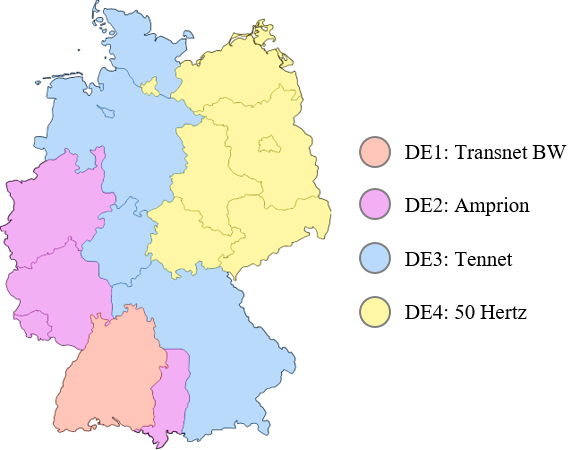
\includegraphics[width=0.6\textwidth]{Regelzonen.png}
    \caption{Control Areas (CA) in Germany.}
    \label{fig:CA_Germany}
\end{figure}

The intraday market serves as last option for trading before delivery and facilitates the balancing of short-term deviations between the submitted schedules of the participants.
There are three different product types on the intraday market to balance short-term deviations: one-hour, half-hour and quarter-hour products.
Each of these products is characterized by its delivery period of the same name.
As Figure~\ref{fig:Bubblechart} shows, there are three phases on the intraday market, which also restrict the geographical location where trading may take place.
From the start of trading (15:00 pm +01h), contracts can be concluded between all parties, regardless of their location.
This also applies to trading abroad. This phase ends for each product exactly one hour before delivery (gray line, dashed).
From this point onwards, it is only possible to trade nationally. Thirty minutes before delivery, trading is only possible within the four control areas (red line, dashed).

\begin{figure}[h!]
    \centering
    \includegraphics[width=1\textwidth]{SVG/Figure_2.pdf}
    \caption{Average Count of Trades for Quarter Hour Products per Day}
    \label{fig:Trade_occurence}
    \label{fig:Bubblechart}
\end{figure}

While an auction is held once a day on the DAM, at which all prices for the following day are set at the same time, trading on the IDM is continuous.
In this context, continuous means that a bid can be submitted for any product at almost any time from the start of trading, provided it is not in the past \cite{EPEXSPOT.2021b}.
Pricing is carried out using the pay-as-bid method, in which the orders are matched using a matching algorithm.
Price limits are used to determine the price, which are set by the trading participants themselves.
The decisive factor here is whether and on which side of the order book a bid is placed.
If a newly created buy order meets an existing sell order, the limit price of the sell order is used.
If a sell order meets a buy order, the price of the buy limit is used.
In principle, the matching algorithm is always triggered when a new bid is created or when an acute grid requirement arises.
Unmatched bids can either be deleted directly or written to the order book \cite{EPEXSPOT.2021}.
The balancing energy price (reBAP), which is charged to the market participant if there are schedule deviations after delivery despite the intraday market, can be seen as a natural upper limit for the price limits \cite[84, 158]{Wawer.2022}.
This price has been linked to the exchange electricity price since 2020 due to various past incidents, which is intended to ensure grid stability \cite{TSOGermany.2022}.
As the intraday market is the last market before delivery, it is the last opportunity for market participants to balance out their schedule.
This leads to an increase in trading intensity before the time of delivery, as can be seen in Figure 2.
This effect can be explained not only by the threat of penalties, but is also due to lower forecast deviations from RES and improved weather forecasts \cite{Pape.2018}.

Figure~\ref{fig:Trade_occurence} shows the average number of trades per day from October 2021 through December 2024.
As can be seen, activity is highest in the final hours before delivery.
Trading activity remains high even after the close of domestic trading.
It is worth noting the low number of trades in control area DE1, while control areas DE2–DE4 show significantly higher trading activity.
\cite{puć2024} also described that the highest liquidity occurs in the last quarter-hour of each full hour.
This effect is evident here in that trading activity in the last quarter-hours begins noticeably earlier and becomes apparent in stages.
This is most clearly visible between 120 and 60 minutes before delivery.

\subsection{Contribution}
In an ex-post experiment, we want to estimate prices for the last thirty minutes before delivery on the German IDM.
At this point in time, national trading is already restricted so that only trades within the individual control areas can be carried out.
The study is limited exclusively to quarter-hourly products, as we consider them to be crucial for short-term balancing within this short period.
In order to specify the thirty minutes before delivery period in more detail, we use the notation of \cite{Narajewski.2020} and extend it to include the control area:
A volume-weighted price \({}_x^{\;}\!\text{ID}_y^{d,s,a}\) can be formed for a product \(s\) on day \(d\) in a specific control area \(a\).
Here, \(x\) and \(y\) delimit the period of the trades taken into account for this product, where \(x \geq 0\) and \(y > 0\).
\(\mathbb{T}_{x,y}^{d,s,a}\) forms the time window under consideration, which is set to the last 30 minutes before delivery with \(x = 0\) and \(y = 0.5\) in the context of this article.
\begin{equation}
    {}_x^{\;}\!\text{ID}_y^{d,s,a}=\frac{1}{\sum_{k\epsilon {\mathbb{T}}_{x,y}^{d,s,a}} \text{V}_{k}^{d,s,a}}\sum_{k\epsilon {\mathbb{T}}_{x,y}^{d,s,a}}\text{V}_{k}^{d,s,a}\ \text{P}_{k}^{d,s,a}
    \label{eq:Formel1}
\end{equation}

The volume-weighted price ID is formed from the respective volumes V with the corresponding prices P of all contracts \(k\) that were concluded in this period.
According to this notation, the volume-weighted average price for this period can be represented as \({}_{0}^{\;}\!\text{ID}_{0.5}^{d,s,a}\).
The last 5 minutes, in which trading is no longer possible, are excluded in this article, as no data is available for this time span. 
In order to offer economic value for traders decisions for the forecast of \({}_{0}^{\;}\!\text{ID}_{0.5}^{d,s,a}\), the information must be provided in such a way that reactions are possible. 
Thus, we have set a time frame 30 minutes for reactions, so that the forecast must be available one hour before delivery.

\begin{figure}[h!]
    \centering
    \includegraphics[width=1\textwidth]{SVG/Versuchsaufbau-Seite-5.drawio.pdf}
    \caption{Composition of ID1 and ID3 and the Timeframe \({}_{0}^{\;}\!\text{ID}_{0.5}^{d,s,a}\) for every Control Area a.}
    \label{fig:Timeframe}
\end{figure}

For the forecast of the control area-specific intraday prices, a rolling-window approach is used.
Here, a model is trained daily on the basis of the preceding 26 months.
The training window is shifted by one day each day.
The hyperparameter optimization is carried out depending on the model according to cross-validation or on a separate validation period, which directly follows the respective training window.

\section{Related Literature}
\subsection{Short term Electricity Price Forecasting}
There are numerous articles on forecasting electricity prices (EPF) on the spot market.
These differ essentially in terms of the tools selected, the market under consideration and the forecasting objective.
With regard to the tools, there are different approaches to price forecasting.

Traditional approaches here are conventional statistical models, such as linear regression, moving averages or exponential smoothing \cite{Lago.2018,Naumzik.2021, Abunofal.2021, Maciejowska.2022, CantilloLuna.2023}.
These models are still very popular.
However, due to their linear component, they have the disadvantage that they can perform relatively poorly in complex contexts, which is why machine or deep learning models are increasingly coming into focus \cite{Amjady.2006, Lago.2018b, Lago.2021, CantilloLuna.2023}.
Another difference in short-term forecasts lies above all in the market under consideration.
A distinction can usually be made here between the Continuous Intraday Market and the Day-ahead Market.
It is noticeable here that the literature has so far clearly focused on the day-ahead market (Lago et al., 2021).
Regarding the objective of the forecasts, a distinction can be made between simple point forecasts, probabilistic forecasts and path forecasts, with the current trend moving towards probabilistic forecasts \cite{Nowotarski.2018, Ziel.2018, Maciejowska.2022, Marcjasz.2023}.
However, the number of publications for point forecasts is significantly higher, which may also be due to the fact that these are the simplest and most intuitive for estimating electricity prices.
Irrespective of the models, market or forecast target, there has also been significant progress in the area of data preparation and handling.
In particular, regularization techniques should be mentioned here, which are able to carry out variable selection in large amounts of data and thus simplify the models.
Established methods in this area are LASSO (L1) \cite{Narajewski.2020} and Ridge (L2) or extensions such as Elastic Nets \cite{Zou.2005}, which deliver the best results for regression models in the context of day-ahead EPF \cite{Uniejewski.2016}.
Of these methods, however, LASSO in combination with linear regression has established itself as a standard for both day-ahead and intraday \cite{Maciejowska.2022}.

\subsection{Electricity Price Forecasting of quarter-hourly contracts on Intraday Market}
Within the intraday market, a large proportion of publications relate to hourly contracts, while quarter-hourly contracts have been studied less frequently. One reason for this may be, for example, the lower trading volume and associated lower liquidity \cite{Marcjasz.2023b}.
As contracts are traded continuously on the IDM, it is possible that there are several prices for the same product over a period of time. Average prices or volume-weighted average prices are therefore used in the literature to counteract this problem.
An example of volume-weighted prices on the German intraday market is the article by Kath and Ziel, who were the first to focus on volume-weighted quarter-hourly contracts on the German intraday market in 2018 \cite{Kath.2018}.
They used linear regression with elastic nets to estimate prices both on the intraday auction and on the continuous intraday market. For this purpose, they used forecasts for RES and load as well as price information from the DAM as exogenous variables.
Another example of volume-weighted price forecasting is the contribution by Narajewski and Ziel, who forecast the ID3 price of hourly and quarter-hourly intraday contracts using various statistical methods and LASSO for the years 2015 to 2018 \cite{Narajewski.2020}.
They were unable to find a model that outperformed the naïve approach, which they assumed to be a weak form of the market efficiency hypothesis. 
A paper published shortly afterwards by Marcjasz et al. made direct reference to this assumption and undermined the statement by proposing a similar approach that included forecast averaging and thus clearly outperformed the naïve approach \cite{Marcjasz.2020}.
However, this study only showed this for the hourly products.
Another study was conducted by \cite{Kremer.2020}, which extended the quarter-hourly overnight contracts of the intraday market to include additional input variables, such as expected consumption of wind power generation or availability of conventional power plants, in their data set from 2015.
This was based on the approach proposed \cite{Narajewski.2020}.
It is noticeable from the previous contributions that most EPF papers deal with a forecast period before 2019.
To our knowledge, there are only six published papers that estimate energy prices (quarter-hourly or hourly) with more recent price dynamics.
While baseline models for rolling forecasts are discussed in \cite{Hornek.2024}, the remaining five articles focus mainly on probabilistic forecasts \cite{Marcjasz.2023, Marcjasz.2023b, Hirsch.2024, Hirsch.2024b, Nickelsen.2024}.
In particular, modified neural networks are used for this purpose.
Ein neuerer Beitrag von puc et al. \cite{puć2024} beschäftigt sich mit der Prognose von Viertelstundenprodukten auf dem deutschen Intraday-Markt.
Hierbei werden verschiedene Modelle, wie Corrected Support Vector Regression, LASSO und random Forests verglichen.
Die besonderheit liegt hierbei in der hochfrequenten Umgebung und der zugrundeliegenden Methode. 
In mehreren Zeitabschnitten wird in diesem Beitrag minütlich prognostiziert, während die letzten dreißig Minuten vor Auslieferung werden jedoch ausgespart werden.

\subsection{LSTM in the Intraday Market}
As we use LSTMs in this study and have not yet found a literature review for them on the intraday market, we would like to briefly mention them here. In the EPF area, LSTMs were used on both spot markets.
On the day-ahead market, there are significantly more articles on this topic, which were summarized by \cite{Lago.2018b}.
The result of this study is that the articles often do not have a sufficiently large test set and often use inadequate benchmarks. On the intraday market, there are only a few articles dedicated to this tool.
The article \cite{Scholz.2021} should be highlighted here, which used transaction data and the M7 order book to forecast the 15-minute contracts on the German intraday market in June 2018.
They used comparison algorithms such as Random Forest or XGBoost. A comparison to the naïve approach, as in \cite{Marcjasz.2020,Narajewski.2020} was not made.
A more recent paper \cite{Klc.2024} also uses LSTMs and deals with price forecasting within DK1, a Danish control area. 
Here, they forecast the hourly intraday prices over a period of slightly less than one month in 2019.
Although this paper does not deal with the German intraday market, it comes quite close to the topic of this paper by applying it to a control area.
For both papers, it should be noted that the respective test period is quite small.
To the best of the authors' knowledge, there are no comparable studies to date that have carried out the IDM prices for a similar period and at delivery area level in Germany.

\section{Data and Benchmarks}
The data for this study comes from various sources.
The most important source for spot prices is EPEX Spot.
In addition, the API of Entsoe and netztransparenz.de provide essential data on generation forecasts or balancing energy.
The Fraunhofer Institute's website, energy-charts.info, was used to validate the data. 
The data on the German electricity market for the period between 2021 and 2024 is characterized by a high price level in particular in late 2021 and during 2022.

\begin{figure}[h!]
    \centering
    \includegraphics[width=1\textwidth]{SVG/Figure_1.pdf}
    \caption{Price Development of the Intraday Auction Price in Germany from October 2021 to December 2024.}
    \label{fig:Price_Development}
\end{figure}

The dataset begins on 1st October 2021 at 12am (30. September 2021, 22:00:00 UTC) and ends on 31th December 2024 at 11:45pm.
The first selected test interval is the 1st January 2024 00:00 to 23:45 and thus contains 96 rows.
The corresponding training set covers the period from 1st October 2021, to November 30, 2023.
The month of December is reserved for validation purposes.
Table 1 lists the data used for the experiment. 
It is important to note that most attributes are differentiated by control zone.
This means that models receive both national indicators and specific data for the control zone currently under consideration.
We compile a single comprehensive input dataset combining historical prices, market activity, balancing energy, commercial balances, as well as national and control area-specific load and generation data (solar, wind onshore, wind offshore).

\begin{table}[htbp]
    \centering
    \caption{Overview of Feature Categories in the Input Dataset.}
    \label{tab:scenarios_overview}
    \small
    \begin{tabular}{llr}
        \toprule
        \textbf{Category} & \textbf{Description} & \textbf{Scope} \\
        \midrule
        \textbf{Target} \cite{EPEXSPOT.2024} & ID price (0--30 min before delivery) & CA-specific \\
        \textbf{Price History} \cite{EPEXSPOT.2024} & DA/ID auction \& ID prices (360--90 min) & National \& CA-specific \\
        \textbf{Time Indicators} & Weekday dummies \& time categories & Global \\
        \textbf{Balancing Energy} \cite{Netztransparenz.2024} & mFRR \& aFFR pos./neg. & National \& CA-specific \\
        \textbf{Load \& Generation} \cite{entsoe.2023} & Actuals, forecasts \& diffs for Load, Solar, Wind & National \& CA-specific \\
        \textbf{Trading Volume \& Activity} \cite{EPEXSPOT.2024} & Aggregated ID volume \& trade count (15-min) & National \& CA-specific \\
        \textbf{Commercial Balance} \cite{EPEXSPOT.2024} & Cross-zonal trade \& self-trades & Per CA pair \\
        \bottomrule
    \end{tabular}
\end{table}

Instead of the real value of the label \({}_0^{\;}\!\text{ID}_{0.5}^{d,s,a}\), we also use its difference to the naïve approach. This is composed as follows:
\begin{equation}
    label\left({}_{0}^{\;}\!\text{ID}_{0.5}^{d,s,a}\right)={}_{0}^{\;}\!\text{ID}_{0.5}^{d,s,a}-{}_{1.5}^{\;}\!\text{ID}_{0.25}^{d,s,a}
    \label{eq:Formel2}
\end{equation}

\section{Data Preparation}
\label{sec:DataPreparation}

The construction of reliable forecasts requires careful data preparation, especially when deep learning models are employed, since these architectures are particularly sensitive to the scale of input variables
\cite{Lago.2018}.
Because we employ a rolling-window scheme that produces 366 individual models per control area, a robust, automated preprocessing pipeline is essential.
All preprocessing steps are implemented in Python using \texttt{scikit-learn} \cite{Pedregosa.2011} and, where applicable, in \texttt{Keras} \cite{chollet2015keras}.
The following subsections describe the pipeline's key components in the order they are applied within each rolling window.

\subsection{Temporal Data Splitting and Leakage Prevention}
\label{sub:TemporalSplit}

For each rolling window, the data is split into three consecutive, non-overlapping time intervals:
\begin{itemize}[noitemsep]
    \item The training set covers 26 months ending on November 30, 2023, with the exact length growing from October 1, 2021 onwards.
    \item The validation set consists of December 2023 (31 days), immediately following the training period.
    \item The test set comprises a single day (96 quarter-hourly observations).
\end{itemize}

This strict temporal ordering is crucial for out-of-sample evaluation: all transformation parameters (scaling, imputation values) are computed exclusively on the training set and then applied to validation and test sets without modification.
This prevents look-ahead bias, where future information would inadvertently leak into the model through the preprocessing steps.

The rolling nature of the experiment means that each daily window receives its own instance of the entire preprocessing pipeline.
This design choice has two implications: (1) it adapts to distribution shifts over time, such as the dramatic price regime change during the 2021--2022 energy crisis, and (2) it keeps the scaling consistent within each window's training distribution.

\subsection{Missing Value Handling}
\label{sub:Imputation}

Continuous intraday trading produces irregularly-spaced transactions, which means that after aggregating into quarter-hourly periods, missing values occur frequently for low-liquidity products.
We handle these in two stages, both applied separately to training, validation, and test sets:

\begin{itemize}[noitemsep]
    \item Prices. Identified by a common prefix price columns are sorted by their time window in descending order and filled with the last known price. 
    The least known Price column (\({}_{5.75}^{\;}\!\text{ID}_{0.25}^{d,s,a}\)) is filled with the Intraday Auction Price if necessary.
    This is also applied to the target variable.
    \item Non-price features. Trading volume and number of trades are filled with zero, reflecting the absence of market activity. Forecast errors and balancing features get filled with the last known value.
\end{itemize}

All imputation steps are completed before the label differencing and scaling stages.

\subsection{Label Differencing and Shifting}
\label{sub:LabelDifferencing}

Before scaling, both the target and certain features are transformed to account for temporal delays in data availability.
First, all input features are aligned with the forecast horizon via lagging.
Hierbei wurden die Lags wie in Abbildung~\ref{fig:Timeframe} dargestellt, gewählt, sodass die Features zum Zeitpunkt der Prognose verfügbar sind.

Second, the target variable is transformed into a price difference to the last known price (na\"ive), as described in Equation~\ref{eq:Formel2}.
However, the label itself is not scaled the differenced price is used directly as the regression target, preserving its interpretability in EUR/MWh.
Hierbei weichen wir von verwandten Beiträgen, wie \cite{Narajewski.2020, puć2024}, ab, die den differenzierten Preis ebenfalls skalieren.

\subsection{Feature Scaling}
\label{sub:Scaling}

The central data preparation step involves scaling the feature matrix.
The scaling is performed after all imputation and transformation steps have been completed.

The scaling procedure consists of two consecutive steps that are applied to the training set: (1) quantile-based clipping (described in Section~\ref{sub:Clipping}), and (2) linear transformation to a standardized range.
For the validation and test sets, only step (2) is applied using the pre-fitted scaler parameters from the training set.

\paragraph{Scaler Types}
We consider two commonly used scaling methods, both implemented via \texttt{scikit-learn} \cite{Pedregosa.2011}:

\begin{itemize}[noitemsep]
    \item \textbf{Min-max Normalization,} which maps each feature to the interval \([0,1]\) via
    \begin{equation}
        x_{\text{scaled}} = \frac{x - \min(x)}{\max(x) - \min(x)}
    \end{equation}
    where \(\min(x)\) and \(\max(x)\) are computed from the training set only.
Min-max normalization is particularly suited for neural networks using sigmoid activations, as it ensures that input values lie within the active region of these functions.
In this case, we also use this scaling for neural networks and LSTM models.

\bigskip

    \item \textbf{Standardization} (Z-score Normalization), which centers each feature at zero with unit variance:
    \begin{equation}
        x_{\text{scaled}} = \frac{x - \mu}{\sigma}
    \end{equation}
    where \(\mu\) and \(\sigma\) are the mean and standard deviation computed from the training set.
    This approach is particularly suitable for linear models and tree-based models like XGBoost, as these models are not sensitive to the absolute scale of the features.
    This scaling is applied to the linear models and XGBoost models.

\end{itemize}

Both scaling methods are parametrized exclusively from the training data within each rolling window.
For the validation and test sets, the scaler is not re-fitted. Instead, the pre-trained transformation is applied directly on both sets.
This ensures that the model's performance on the test set reflects a true out-of-sample scenario where all parameters are determined before the forecast is made.

\subsection{Quantile-Based Clipping}
\label{sub:Clipping}

Electricity prices are notoriously prone to extreme outliers, including negative price spikes during periods of excess renewable generation and scarcity pricing during supply crunches.
\cite{Janczura.2013} note that spike identification is one of the primary challenges in electricity price modeling.
In the context of min-max normalization, even a single extreme value in the training set would compress the remaining data into a very narrow range of \([0,1]\).
This effect is particularly problematic for network models, where the gradient flow through sigmoid activations would be severely diminished by inputs clustered at the edges of their active regions \cite{Lago.2018}.
To address this, we apply a subtle form of outlier control, which we refer to as \emph{quantile-based clipping}, before fitting the scaler.

For each feature column \(c\) in the training set, we compute the lower and upper quantiles:
\begin{equation}
    lo_c = Q_c(q)
    \quad \text{and} \quad
    hi_c = Q_c(1 - q)
\end{equation}
where \(Q_c(\alpha)\) denotes the \(\alpha\)-quantile of feature \(c\) and \(q\) is a pre-specified clipping threshold.
Each feature is then clipped to the computed bounds:
\begin{equation}
    x_c \equiv \operatorname{clip}(x_c, lo_c, hi_c) = \begin{cases}
            lo_c, & x_c < lo_c \\
            x_c, & lo_c \leq x_c \leq hi_c \\
            hi_c, & x_c > hi_c
          \end{cases}
\end{equation}

In our experiments, we set \(q = 0.01\), which clips the bottom 1\% and top 1\% of each feature's distribution.
This threshold is chosen as a balance between two conflicting goals: (1) the clipping should be strict enough to prevent extreme values from dominating the scaling, but (2) it should be permissive enough to preserve the full range of normal price variation, especially during volatile periods.
The clipping bounds \(lo_c\) and \(hi_c\) are not applied to validation and test data. This is intentional: the clipping is a training-only regularization technique that prevents the scaler from being distorted by extreme training values. 
On validation/test data, the fitted scaler will map values outside the training range to values outside \([0,1]\) for Min-Max scaling, which is appropriate. 
These observations are genuinely in a regime that was not present in the training data and the model should treat them as such.

\subsection{Sequence Construction for RNN Models}
\label{sub:Sequences}

As a final transformation step, we convert the 2D feature matrix into a 3D tensor required by the LSTM architecture \cite{Hochreiter.1997}.
Going from a flat feature matrix \(\mathbb{R}^{N \times f}, (N \times f)\) to a sequence tensor \((N \times s \times f)\), each sample includes the previous \(s\) time steps:
\begin{equation}
    \mathbf{X}^{\text{seq}}_{i} = \big(\mathbf{x}_{i-s}, \mathbf{x}_{i-s+1}, \dots, \mathbf{x}_{i-1}, \mathbf{x}_{i}\big)^{\top}
    \label{eq:sequences}
\end{equation}
Where \(\mathbf{x}_{i} \in \mathbb{R}^{f}\) denotes the feature vector at time step \(i\), \(s\) is the sequence length. \(s = 0\) is set for non-recurrent models (Feedforward Neural Network, XGBoost, LASSO, Linear Regression), which operate directly on the flat feature matrix without temporal context.

The sequence construction is performed after all previous preprocessing steps have been completed and independently for training, validation, and test sets.
It is worth noting that this transformation reduces the number of samples from \(N\) to \(N - s\), which means that the sequence length must be balanced against the available training data.
For our experiment, with a 26-month training window (approximately 57,000 quarter-hourly observations), even a sequence length of \(8 \times 15\text{ minutes} = 2\text{ hours}\) leaves sufficient training samples.
However, the trade-off between sequence length and sample size becomes more pronounced for the validation set (31 days) or the test set (1 day), where sequence-based predictions may be computationally challenging.

\subsection{Further Input Attributes}
The commercial balance between the control areas is another indicator that we would like to include in the forecast.
For this, the EPEX data can be used to determine the trade balance for each control area.
This makes it possible to determine whether a control area is over- or under-covered, at least from the perspective of the trades executed.
In order to carry out these calculations, the trades for each control area were divided into three different categories: Import, Export and Self-Trade.
The latter describes a trade that was only carried out within the control area in question and can basically occur at any time.
The fact that the national trades in the raw data usually occur in pairs (buy and sell) was utilized here.
The categories were thus formed successively for each control area according to the following rules:
\begin{enumerate}[noitemsep]
    \item Only trades in which the current delivery area (control area) is involved are considered.
    \item Only trades with the same TradeID are matched in pairs.
    \item If the delivery area of one of the two orders does not correspond to the currently considered control area and this entry is a ``Buy'', the ``Export'' category is formed.
    \item If the delivery area of one of the two orders does not correspond to the control area currently under consideration and this entry is a ``Sell'', the ``Import'' category is created.
    \item If both TradeIDs correspond to the delivery area under consideration, it is a self-trade.
\end{enumerate}

\begin{table}[htbp]
    \centering

    \caption{Balance (in MWh) of 15 minute Products 180 to 30 Minutes before Delivery. \\ (row – from | column – to; exports considered as negative values) \\ DE1: Transnet BW, DE2: Amprion, DE3: Tennet, DE4: 50Hertz.}
    \label{tab:trade_balances_formatted}
    \setlength{\tabcolsep}{4pt}
    \small
    \renewcommand{\arraystretch}{0.85}
    \begin{tabular}{llrrrr}
        \toprule
        & \textbf{Control Area} & \textbf{DE1} & \textbf{DE2} & \textbf{DE3} & \textbf{DE4} \\
        \midrule
        \multicolumn{6}{l}{\textbf{Year 2021} \textit{(92 available days)}} \\[0.1cm]
        & \textbf{DE1} & -- & 5,801.10 & 9,497.73 & 6,463.43 \\
        & \textbf{DE2} & -5,801.10 & -- & 12,900.95 & -397.55 \\
        & \textbf{DE3} & -9,497.73 & -12,900.95 & -- & -7,048.15 \\
        & \textbf{DE4} & -6,463.43 & 397.55 & 7,048.15 & -- \\
        \addlinespace
        \multicolumn{6}{l}{\textbf{Year 2022} \textit{(365 available days)}} \\[0.1cm]
        & \textbf{DE1} & -- & -24,945.83 & -25,955.17 & 3,154.12 \\
        & \textbf{DE2} & 24,945.83 & -- & 20,685.35 & 39,435.82 \\
        & \textbf{DE3} & 25,955.17 & -20,685.35 & -- & 11,119.52 \\
        & \textbf{DE4} & -3,154.12 & -39,435.82 & -11,119.52 & -- \\
        \addlinespace
        \multicolumn{6}{l}{\textbf{Year 2023} \textit{(365 available days)}} \\[0.1cm]
        & \textbf{DE1} & -- & -37,119.68 & -28,659.17 & -32,158.20 \\
        & \textbf{DE2} & 37,119.68 & -- & 24,615.75 & 27,178.17 \\
        & \textbf{DE3} & 28,659.17 & -24,615.75 & -- & -4,538.25 \\
        & \textbf{DE4} & 32,158.20 & -27,178.17 & 4,538.25 & -- \\
        \addlinespace
        \multicolumn{6}{l}{\textbf{Year 2024} \textit{(366 available days)}} \\[0.1cm]
        & \textbf{DE1} & -- & -19,758.25 & -15,758.55 & -8,602.70 \\
        & \textbf{DE2} & 19,758.25 & -- & 17,636.10 & 9,340.50 \\
        & \textbf{DE3} & 15,758.55 & -17,636.10 & -- & 24,866.22 \\
        & \textbf{DE4} & 8,602.70 & -9,340.50 & -24,866.22 & -- \\
        \bottomrule
    \end{tabular}
\end{table}
An overview of the calculated balance for the 15-minute products for each control area from 360 to 30 minutes before delivery can be found in Table \ref{tab:trade_balances_formatted}.
Of course, this procedure does not determine the actual surplus or shortfall in the control area.
In addition, a test with the balancing energy used only shows a low negative correlation between the trading balance and the balancing energy used.
However, we consider the quantity traded between the control areas to be a crucial feature for subsequent forecasts.

When constructing forecasts, only the data available at the time of forecasting can be used.
According to ENTSO-E, all considered exogenous data is available no later than one hour after the end of the application period.
The delay in continuous intraday data availability on EPEX SPOT sFTP server is 20 minutes.
Netztransparenz.de typically publishes its data for balancing energy 15 minutes after the product expires.
We use the operational data here, since the quality-assured data isn't published until 20 days later.
%https://www.netztransparenz.de/xspproxy/api/staticfiles/ntp-relaunch/dokumente/regelenergie/regelenergie%20(%C3%BCs)/rl-erlaeuterungen_ntp_20230710.pdf
Hence, we set the delay for intraday exogenous information used in the model and prices accordingly.

\section{Models}
Our study includes a high number of individual point forecasts, since we make forecasts for each of the four control zones (DE1–DE4) separately. 
This increases the computational burden, especially for the more complex models, like NN and LSTM.
These models are both considerably more expensive to train and tune than traditional methods.
Therefore, method selection must strike a pragmatic balance between predictive accuracy and computational feasibility. The experiment was executed on two physical devices:
processor optimized models, such as XGB, LR, and LASSO, were run on Windows 10 on an AMD Ryzen 7700X using the Concurrent package \cite{PythonConcurrentFutures}, while NN and LSTM were run sequentially on an RTX 3060 12GB in an Ubuntu environment.
The Keras framework \cite{chollet2015keras} was used for the network architectures.
Below, we provide a short overview of the theoretical background of each method, discuss their respective strengths and limitations in our setting, and how their Hyperparameters got optimized.
Hyperparameter optimization is model-dependent.
Validation always takes place over a separate time period that immediately follows the respective training window (December 2023).
For models with continuous hyperparameter spaces, Bayesian optimization using Gaussian processes is employed (\texttt{scikit-optimize}, \cite{Bergstra.2011}).

To address the challenges of non-stationarity and structural regime shifts in intraday electricity markets, we incorporate Model-Agnostic Meta-Learning (MAML) \cite{Finn.2017} into our neural forecasting architectures.
Rather than optimizing model parameters for static performance across all historical periods, MAML explicitly trains a meta-initialization $\theta$ that resides in a parameter space highly sensitive to local market conditions. This sensitivity allows the network to achieve remarkable flexibility through minimal adaptation.

The meta-learning process partitions continuous time series into discrete daily tasks $T_i = (S_i, Q_i)$, defined as follows:
\begin{itemize}
    \item \textbf{Support Set ($S_i$):} The $96$ quarter-hourly observations of day $k$ used during the \textit{inner loop} to adapt the meta-weights $\theta$ to task-specific parameters $\theta'_i$.
    \item \textbf{Query Set ($Q_i$):} The $96$ quarter-hourly observations of the subsequent day $k+1$ used during the \textit{outer loop} to evaluate the generalization performance of $\theta'_i$ and update the global meta-initialization $\theta$.
    \item \textbf{Step Size ($\alpha$) and Adaptation Steps ($K$):} The inner-loop learning rate $\alpha$ controls the magnitude of parameter updates per step, while $K$ specifies the number of sequential gradient updates ($\theta'_i = \theta - \alpha \sum_{j=1}^{K} \nabla_\theta \mathcal{L}_{S_i}$).
\end{itemize}
This bi-level structure ensures that the neural network learns \textit{how to adapt} rapidly, enabling sub-second online calibration to intraday price shifts on each evaluation day.

\textbf{LASSO.}
The regularization parameter $\alpha$ is determined for each rolling window over 100 trials within the logarithmic interval $[10^{-5}, 2]$.
The one-dimensional search space keeps the computational effort negligible.
L1-penalized regression implements automatic variable selection, by setting irrelevant predictors to zero \cite{Tibshirani.1996}.
This reduces overfitting in high-dimensional feature spaces and improves interpretability, since only a subset of the predictors is included in the final model.
LASSO has established itself as a robust benchmark for both day-ahead and intraday forecasts \cite{Uniejewski.2016,Ziel.2016,Narajewski.2020}.
The restriction to additive linear effects remains in place.

\textbf{XGBoost.}
For each training window, five parameters are optimized in 30 trials:
Number of boosting rounds ($50$–$300$), learning rate ($5\times10^{-4}$–$5\times10^{-2}$), column-wise subsampling rate ($0{,} 5$–$1{,}0$), maximum tree depth ($7$–$10$), and L1 regularization ($10^{-5}$–$2{,}0$).
The row-wise subsampling rate is fixed at $1{,}0$.
The gradient boosting ensemble models nonlinear relationships and heterogeneous feature effects without manual transformation \cite{Chen.2016}.
It trains efficiently and is less prone to overfitting on structured data than deep neural networks.
One disadvantage, as with LASSO, NN, and LR, is the lack of support for temporal dependencies in the model architecture.
All temporal structure must be provided via feature engineering (lags), which in turn may lead to a deeper tree and thus potential overfitting.

\textbf{Neural Networks and LSTM (MAML Framework).}
To capture the dynamic regime shifts inherent to intraday electricity markets, we implement Model-Agnostic Meta-Learning (MAML) \cite{Finn.2017} for both neural network architectures (Feed-Forward NN and LSTM).
Rather than training a rigid predictive model, MAML optimizes a meta-model initialization that rapidly adapts to recent market conditions via a few gradient steps on the support set (most recent day) to forecast the query set (subsequent day).

Hyperparameter optimization is governed by an automated \textit{Champion-vs-Challenger} mechanism executed periodically every 30 days:
\begin{itemize}
    \item \textbf{MAML Feed-Forward NN:} The search space optimizes first-layer units ($32$--$512$), second-layer units ($16$--$256$), dropout rates ($0$--$0.4$), inner learning rates ($10^{-4}$--$10^{-2}$), outer learning rates ($10^{-4}$--$10^{-2}$), and inner-loop adaptation steps ($1$--$8$).
    \item \textbf{MAML LSTM:} The recurrent architecture models temporal sequences. In addition to hidden units ($32$--$512$ / $16$--$256$), dropout rates, and learning rates, the search space incorporates the optimal temporal lookback horizon ($1$--$24$ quarter-hours).
\end{itemize}
Bayesian optimization (\texttt{skopt.gp\_minimize}) is performed over 5 trials, each consisting of 5 meta-epochs. Every 30 days, the newly tuned challenger model is evaluated against the prevailing champion model on the validation set. The challenger replaces the champion only if it yields a lower Mean Absolute Error (MAE).
On regular evaluation days between 30-day retuning intervals, the meta-weights are retained and adapted daily in milliseconds via 5 gradient steps on the preceding 96 quarter-hours.

\subsection*{Computational Complexity Analysis of FOMAML Meta-Epochs}
To formalize the computational overhead of First-Order Model-Agnostic Meta-Learning (FOMAML) \citep{Finn.2017,Nichol.2018} compared to standard gradient-based neural network optimization, we quantify the gradient operations per epoch. 
Let $\mathcal{D} = \{T_1, T_2, \dots, T_M\}$ denote the set of $M = 780$ daily rolling window tasks generated from $N_{\text{total}} = 75,000$ quarter-hourly electricity price observations. In standard supervised training with mini-batch size $b = 64$, one epoch consists of $N_{\text{std}}$ first-order gradient passes:
\begin{equation}
    N_{\text{std}} = \left\lceil \frac{N_{\text{total}}}{b} \right\rceil = 1,172 \quad \text{gradient evaluations.}
\end{equation}
While full MAML backpropagates through the inner adaptation graph via Vector-Hessian Products:
\begin{equation}
    \nabla_{\theta} \mathcal{L}_{Q_i}(\theta'_i) = \nabla_{\theta'_i} \mathcal{L}_{Q_i}(\theta'_i) \cdot \left( I - \alpha \sum_{k=1}^{K} \nabla_{\theta}^2 \mathcal{L}_{S_i}(\theta_{k-1}) \right),
\end{equation}
FOMAML \cite{Finn.2017,Nichol.2018} eliminates second-order derivatives by approximating the Jacobian $\frac{\partial \theta'_i}{\partial \theta} \approx I$, resulting in the first-order meta-gradient:
\begin{equation}
    g_{\text{FOMAML}} = \sum_{i=1}^{M} \nabla_{\theta'_i} \mathcal{L}_{Q_i}(\theta'_i),
\end{equation}
where $\theta'_i = \theta - \alpha \sum_{k=1}^{K} \nabla_{\theta} \mathcal{L}_{S_i}(\theta_{k-1})$ represents the task-adapted weights after $K = 5$ inner steps.
Executing a single FOMAML meta-epoch over all $M = 780$ daily tasks requires $K = 5$ inner adaptation steps plus 1 outer query evaluation per task:
\begin{equation}
    N_{\text{FOMAML}} = M \cdot (K + 1) = 780 \cdot (5 + 1) = 4,680 \quad \text{first-order gradient evaluations.}
\end{equation}
Consequently, the floating-point operations (FLOPs) of one FOMAML meta-epoch relative to standard training yield:
\begin{equation}
    \text{FLOP Ratio (per meta-epoch)} = \frac{N_{\text{FOMAML}}}{N_{\text{std}}} = \frac{4,680}{1,172} \approx 3.99 \quad \text{standard training epochs.}
\end{equation}
Thus, a single FOMAML meta-epoch requires roughly $4\times$ the computation of a standard training epoch. Executing a full training run of $E_{\text{meta}} = 5$ meta-epochs is computationally equivalent to approximately $20$ standard training epochs on continuous tabular features.

\textbf{Linear Regression.}
\texttt{LinearRegression} From \texttt{scikit-learn}, \cite{Pedregosa.2011}, it does not require any hyperparameters.
It is expected that LASSO will outperform it here.

\textbf{Naïve Approach.}
The volume-weighted price of the ${}_{1{,}5}^{\;}\!\text{ID}_{0{,}25}^{d,s,a}$ window (90–105 minutes before delivery) serves as a lower reference.
\cite{Narajewski.2020} interpret the strength of this benchmark on the German IDM as a weak form of the market efficiency hypothesis. \cite{Marcjasz.2020} have already shown that it can be outperformed by forecast averaging.

\section{Results}
Für die Auswertung der Ergebnisse werden die relative Werte, wie rMAE und rRMSE verwendet.
Diese werden wie folgt berechnet:
\begin{equation}
    rMAE = \frac{MAE_{Model}}{MAE_{Naive}}
\end{equation}
\begin{equation}
    rRMSE = \frac{RMSE_{Model}}{RMSE_{Naive}}
\end{equation}

% ── BLEND VS NAÏVE BENCHMARK TABELLE (ALL ZONES INKL. RANKING) ──
\begin{table}[ht]
\centering
\caption{50/50 Blend vs. Na\"ive Benchmark Performance and Rankings across Control Zones}
\label{tab:blend_vs_bm_all_zones}
\small
\begin{tabular}{llcrrrrr}
\toprule
Zone & Model & Rank & $\bar{\text{MAE}}$ & DM $t$ & $p$-val & GW $\chi^2$ & $N$ \\
\midrule
    \textbf{DE1} & Na\"ive BM & 4 & 26.316 & — & — & — & 366 \\
                 & LR       & \textbf{1} & \textbf{25.464} & +4.983 & $0.0000^{***}$ & +24.829 & 366 \\
                 & LASSO    & 2 & 26.003 & +5.059 & $0.0000^{***}$ & +25.597 & 366 \\
                 & XGB      & 5 & 26.320 & -0.120 & $0.9042$ & +0.014 & 366 \\
                 & NN       & 3 & 26.187 & +1.803 & $0.0715^{*}$ & +3.249 & 366 \\
                 & LSTM     & 6 & 26.604 & -3.308 & $0.0009^{***}$ & +10.941 & 366 \\
    \midrule
    \textbf{DE2} & Na\"ive BM & 4 & 26.688 & — & — & — & 366 \\
                 & LR       & 2 & 26.453 & +1.515 & $0.1298$ & +2.295 & 366 \\
                 & LASSO    & \textbf{1} & \textbf{26.401} & +4.355 & $0.0000^{***}$ & +18.969 & 366 \\
                 & XGB      & 5 & 26.703 & -0.606 & $0.5444$ & +0.368 & 366 \\
                 & NN       & 3 & 26.529 & +2.277 & $0.0228^{**}$ & +5.186 & 366 \\
                 & LSTM     & 6 & 27.748 & -5.477 & $0.0000^{***}$ & +29.998 & 366 \\
    \midrule
    \textbf{DE3} & Na\"ive BM & 4 & 27.284 & — & — & — & 366 \\
                 & LR       & \textbf{1} & \textbf{26.871} & +2.584 & $0.0098^{***}$ & +6.678 & 366 \\
                 & LASSO    & 2 & 27.045 & +3.641 & $0.0003^{***}$ & +13.255 & 366 \\
                 & XGB      & 5 & 27.313 & -0.958 & $0.3381$ & +0.918 & 366 \\
                 & NN       & 3 & 27.145 & +3.209 & $0.0013^{***}$ & +10.298 & 366 \\
                 & LSTM     & 6 & 28.337 & -5.492 & $0.0000^{***}$ & +30.160 & 366 \\
    \midrule
    \textbf{DE4} & Na\"ive BM & 4 & 27.258 & — & — & — & 366 \\
                 & LR       & 2 & 27.027 & +1.562 & $0.1182$ & +2.441 & 366 \\
                 & LASSO    & \textbf{1} & \textbf{26.898} & +3.692 & $0.0002^{***}$ & +13.633 & 366 \\
                 & XGB      & 5 & 27.287 & -1.094 & $0.2739$ & +1.197 & 366 \\
                 & NN       & 3 & 27.151 & +2.250 & $0.0244^{**}$ & +5.064 & 366 \\
                 & LSTM     & 6 & 28.324 & -5.425 & $0.0000^{***}$ & +29.429 & 366 \\
\bottomrule
\end{tabular}
\begin{tablenotes}\small
\item \textit{Note:} 50/50 blend = 0.5 $\times$ model + 0.5 $\times$ na\"ive benchmark. $\bar{\text{MAE}}$ denotes the average daily Mean Absolute Error.
Rankings (1 = best) are computed across all 5 blends and the unblended Na\"ive Benchmark.
DM $t$ and GW $\chi^2$ evaluate the blend against the Na\"ive Benchmark.
$^{***}p<0.01$, $^{**}p<0.05$, $^{*}p<0.10$.
\end{tablenotes}
\end{table}

\section{Proposed Model for parallel Zone Forecasting}
In den letzten Kapiteln führten wir Experimente an vier verschiedenen Datensets durch.
Bei Betrachtung des Einflusses der exogenen Variablen mittels SAGE, sowie die Verbesserung der Ergebnisse durch Forecast Averaging zeigen, dass die Hinzunahme von Daten aus den anderen Regelzonen die Performance verbessern können.
Basierend auf diesen Erkenntnissen erstellen wir im Folgenden einen Modellentwurf, der alle Regelzonen gleichzeitig verarbeitet und prognostiziert.
Da sich in den bisherigen Experimenten das Neuronale Netz als am zuverlässigsten herausgestellt hat, soll dieses für diesen Versuch verwendet werden.
Jedoch hat diese Wahl auch zwei zentrale Nachteile. 
Zum einen kritisiert \cite{puć2024} zurecht die mangelnde Performance von Neuronalen Netzen im Kontext von kurzfristigen Prognosen, aufgrund der langen Trainingszeit.
Insbesondere in noch kürzeren Abständen, sind Neuronale Netze nicht schnell genug für ein vollständiges retraining.

\newpage

\printbibliography

\end{document}
